
\section{Introduction}


\subsection{Goals and motivations}

Inspired by the OLPC web site%
\footnote{Visit the OLPC website at \cite{olpc-website}%
} the vision for the current project was to visualize packets traveling
through a {}``real'' simulated mesh network. The OLPC web site has
a nice Flash based visualization tool which shows possible connections
between multiple laptops forming a common mash network. A screenshot
of this Flash based tool can be seen in figure \ref{fig:OLPC-network-visualization}.

%
\begin{figure}


\begin{centering}
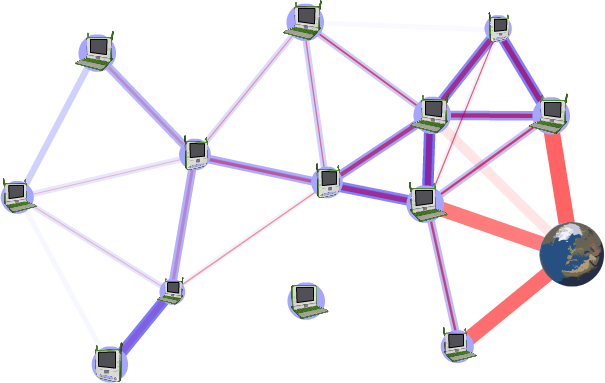
\includegraphics[scale=0.6]{figures/olpc-network}
\par\end{centering}

\caption{\label{fig:OLPC-network-visualization}OLPC network visualization}

\end{figure}


One can drag single laptops on the canvas using the mouse and immediately
observe the effect on the possible connection path changes. The vision
for the current project work was to develop a similar visualization
tool but based on a real network simulation and real packets in order
to be able to observe the choosen routes nearly in realtime.


\subsection{The NS-3 simulator}

The secondary goal was to get accustomed with the NS-3 simulator.
It is supposed to become the successor of the famous NS-2 network
simulator. It is is not backwards compatible and does not rely on
existing NS-2 code. NS-3 is entirely written in C++ and includes state-of-the-art
architectual principles and design patterns. Therefore the current
project work's goal also was to evaluate the usage of the following
technologies supported by NS-3:
\begin{itemize}
\item C++
\item Python
\end{itemize}

